\documentclass[12pt,a4paper]{article}
\usepackage[utf8]{inputenc}
\usepackage[margin=1in]{geometry}
\usepackage{graphicx}
\usepackage{xcolor}
\usepackage{tcolorbox}
\usepackage{tabularx}
\usepackage{booktabs}
\usepackage{enumitem}
\usepackage{hyperref}
\hypersetup{
    colorlinks=true,
    linkcolor=black,
    filecolor=black,
    urlcolor=black,
    citecolor=black
}

\usepackage{listings}

% Define colors
\definecolor{problemred}{RGB}{220,53,69}
\definecolor{solutiongreen}{RGB}{40,167,69}
\definecolor{hciblue}{RGB}{0,123,255}

\title{\textbf{Google Meet Redesign \& HCI Feature Mapping}\\
\large Final HCI Portfolio: Cognitive Comfort, Flexibility, and Error Prevention}
\author{CHALAMCHALA ANJANI NITHIN}
\date{\today}

\begin{document}

\begin{titlepage}
\begin{center}

{\LARGE \textbf{Indian Institute of Information Technology,\\
Design and Manufacturing, Kancheepuram}}\\[1.5cm]

{\large (HCI End-Semester Final Portfolio)}\\[3cm]

\rule{\linewidth}{0.5pt}\\[0.4cm]
{\Huge \textbf{The Google Meet Redesign}}\\[0.3cm]
{\Large \textbf{Cognitive Defense, Deep Heuristic Mapping \& Prototype Realization}}\\[0.3cm]
\rule{\linewidth}{0.5pt}\\[2cm]

\vfill

\textbf{CHALAMCHALA ANJANI NITHIN}\\[0.2cm]
\textbf{CS23B1102}\\[0.2cm]
\textit{Department of Computer Science and Engineering}\\[0.5cm]

{\large \today}

\end{center}
\end{titlepage}

\newpage
\tableofcontents
\newpage

\section{Introduction}

The objective of this final HCI portfolio is to present the complete architectural redesign of the Google Meet platform. Moving beyond traditional "prototype blocks", this report demonstrates fully realized HTML/CSS high-fidelity layouts, providing strict, in-depth mappings between the visual layout and fundamental cognitive design laws, Shneiderman's 8 Golden Rules, and Nielsen's Usability Heuristics.

This iteration pivots to focus heavily on Error Prevention, Learnability, Flexibility, and Persuasion Psychology as directed.

\section{Deep Mapping: HCI Design Laws}

\subsection{Fitts's Law \& The Persistent Control Bar}
Fitts's Law states that the time to acquire a target is a function of the distance to and size of the target. The legacy Google Meet interface auto-hides the control bar after 3 seconds of inactivity, which forces users to "hunt" for controls (increasing distance and cognitive load). 

\textbf{Implementation:} We implemented a \textbf{Persistent Control Bar}. By locking the controls at the bottom edge of the screen, we create an "infinite edge" bounding box, meaning users can impulsively throw their mouse downward and reliably hit the control zone.

\begin{figure}[h]
    \centering
    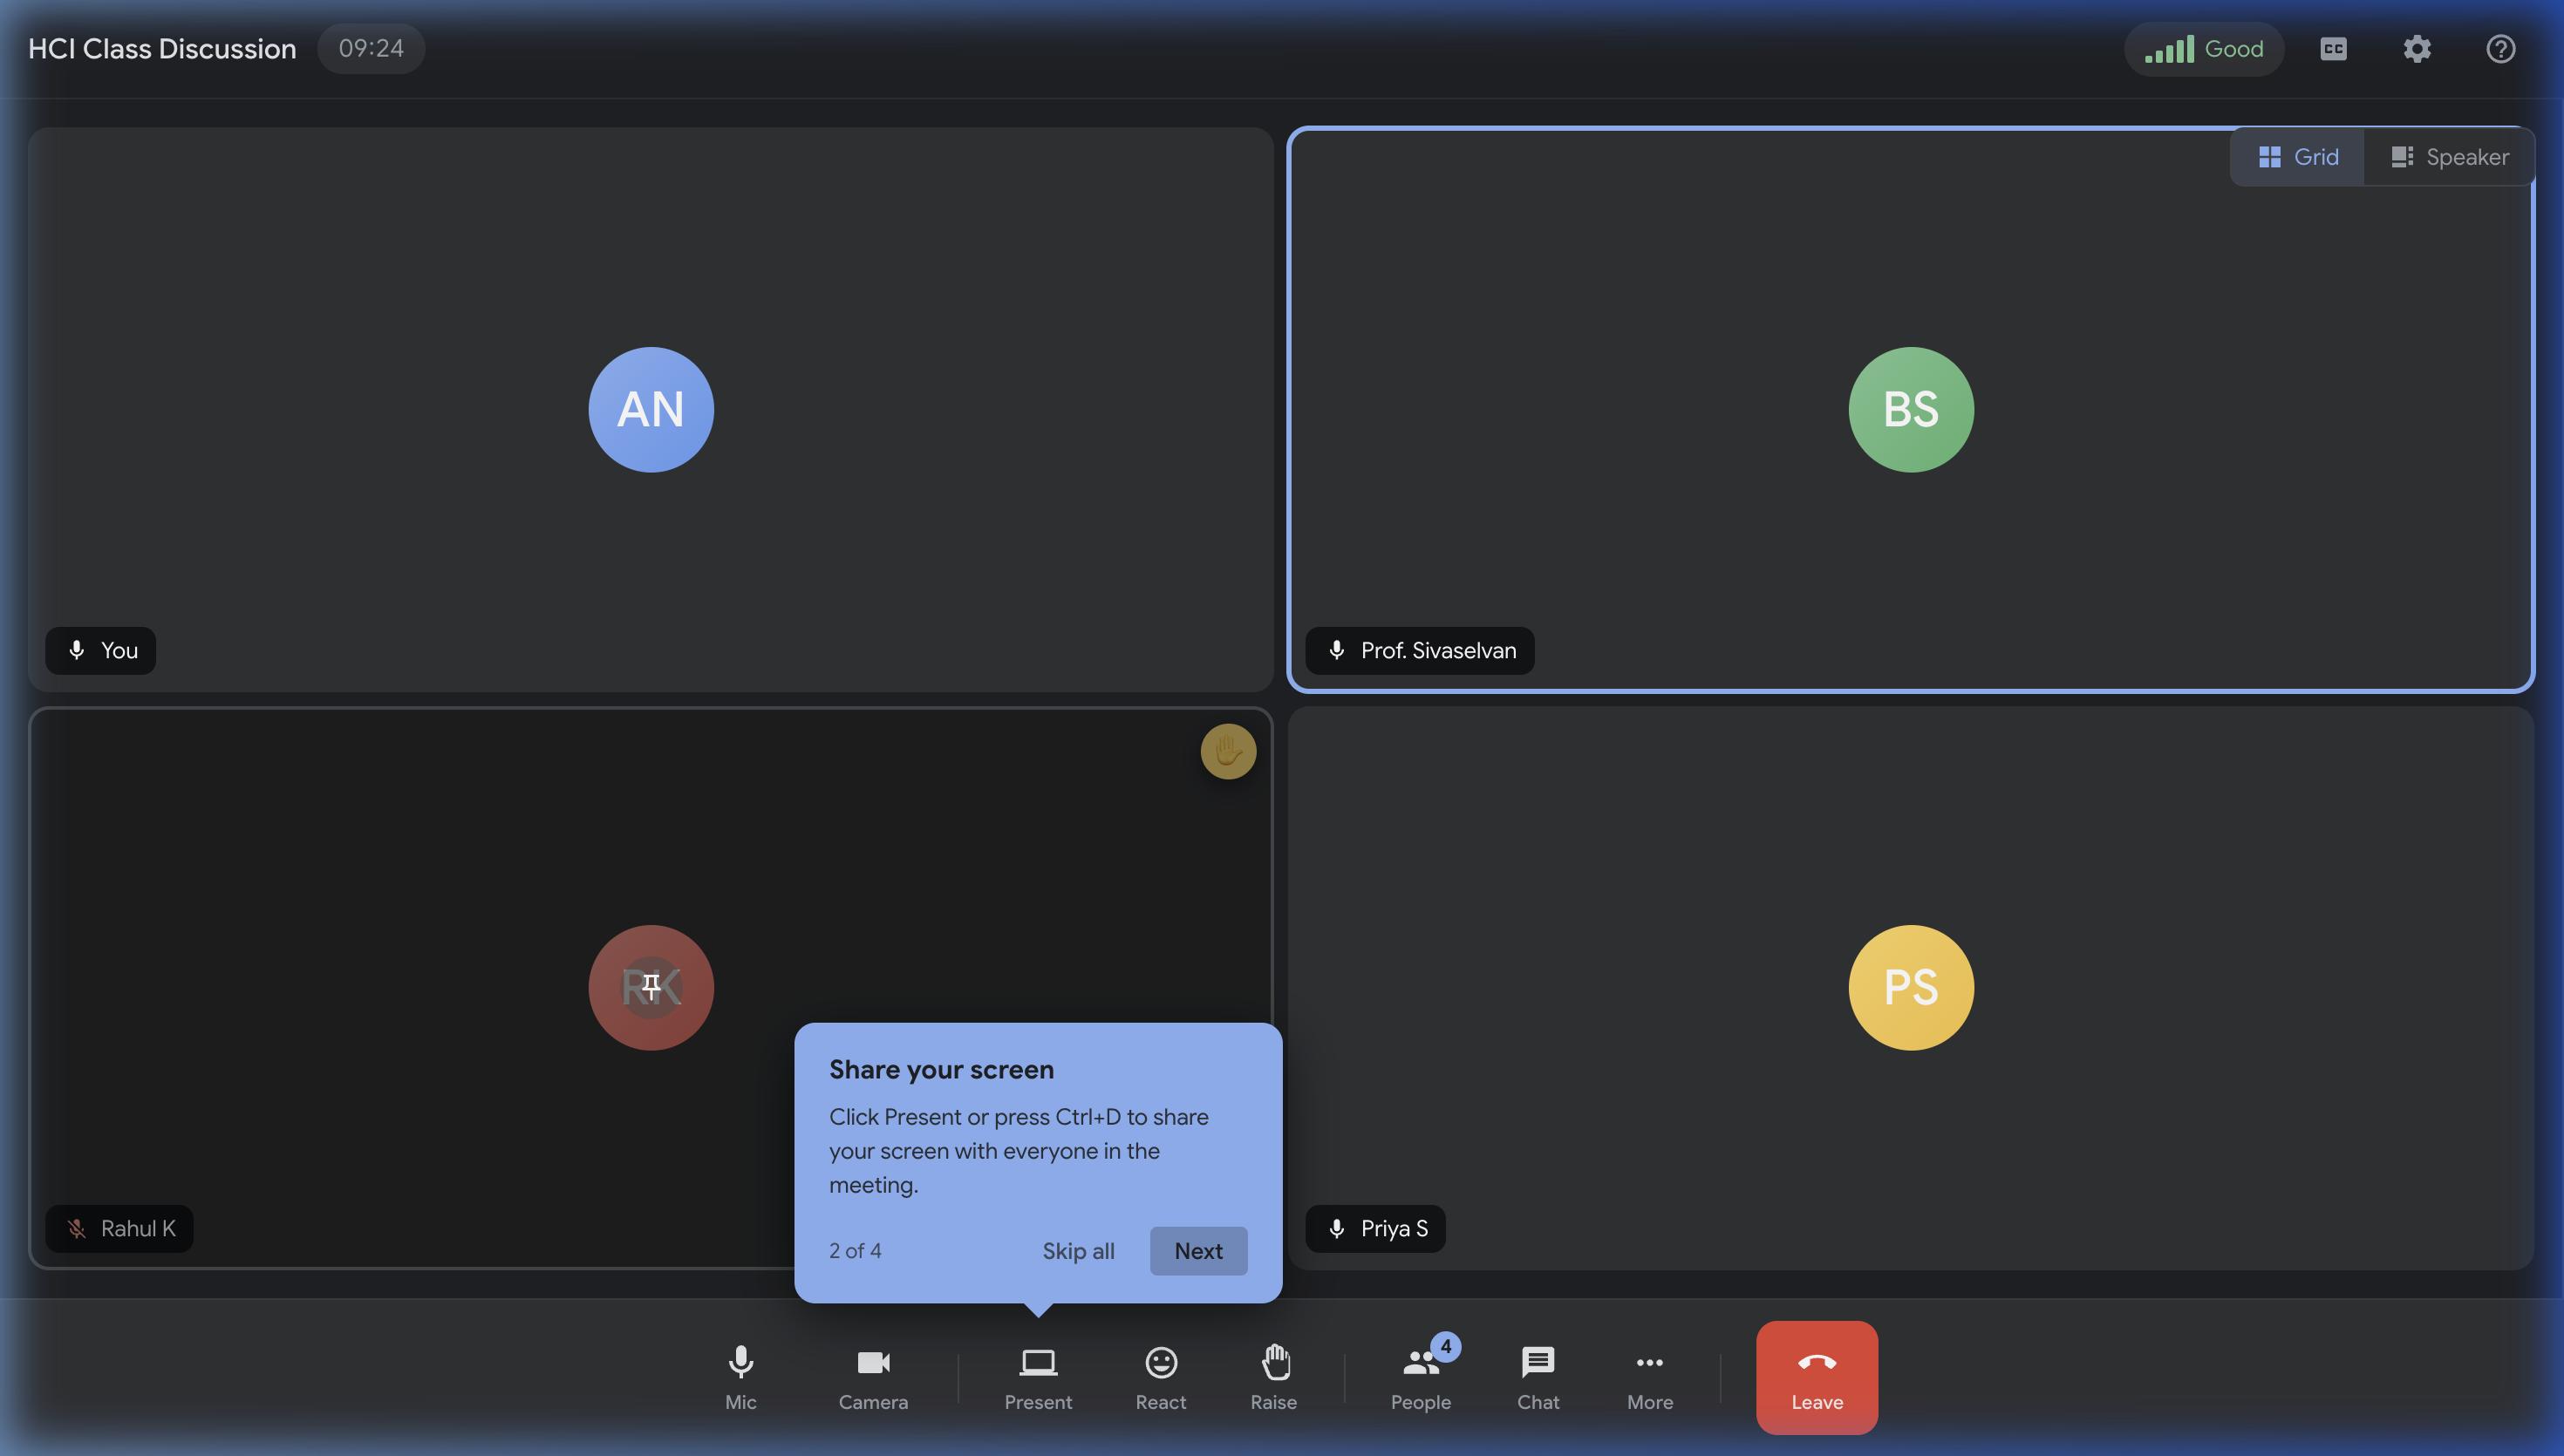
\includegraphics[width=0.8\textwidth]{images/clean_ui.png}
    \caption{Persistent Control Bar ensuring continuous Fitts's Law compliance.}
\end{figure}

\subsection{Hick's Law \& Miller's Law}
Hick's Law bounds the time it takes to make a decision based on the amount of choices, while Miller's Law bounds working memory to $7 \pm 2$ chunks of information.
By stripping the primary control bar to exactly \textbf{7 primary buttons} (Mic, Camera, Screen Share, Hand Raise, Chat, Participants, Leave), we drastically lower the decision-making index.

\newpage
\section{Deep Mapping: Usability Heuristics}

\subsection{Nielsen's Heuristic \#5: Error Prevention}
The most robust design prevents a problem from occurring in the first place, overriding the need for strong error messages.

\subsubsection{The "Leave Meeting" Confirmatory Message}
Accidental meeting exits are a common source of friction. In our redesign, clicking "Leave" no longer instantly terminates the session. Instead, it triggers a \textbf{Confirmatory Message Modal}. The "Stay in Meeting" button is deliberately sized larger (exploiting Fitts's Law) and colored neutrally to prevent catastrophic destructive sequences.

\begin{figure}[h]
    \centering
    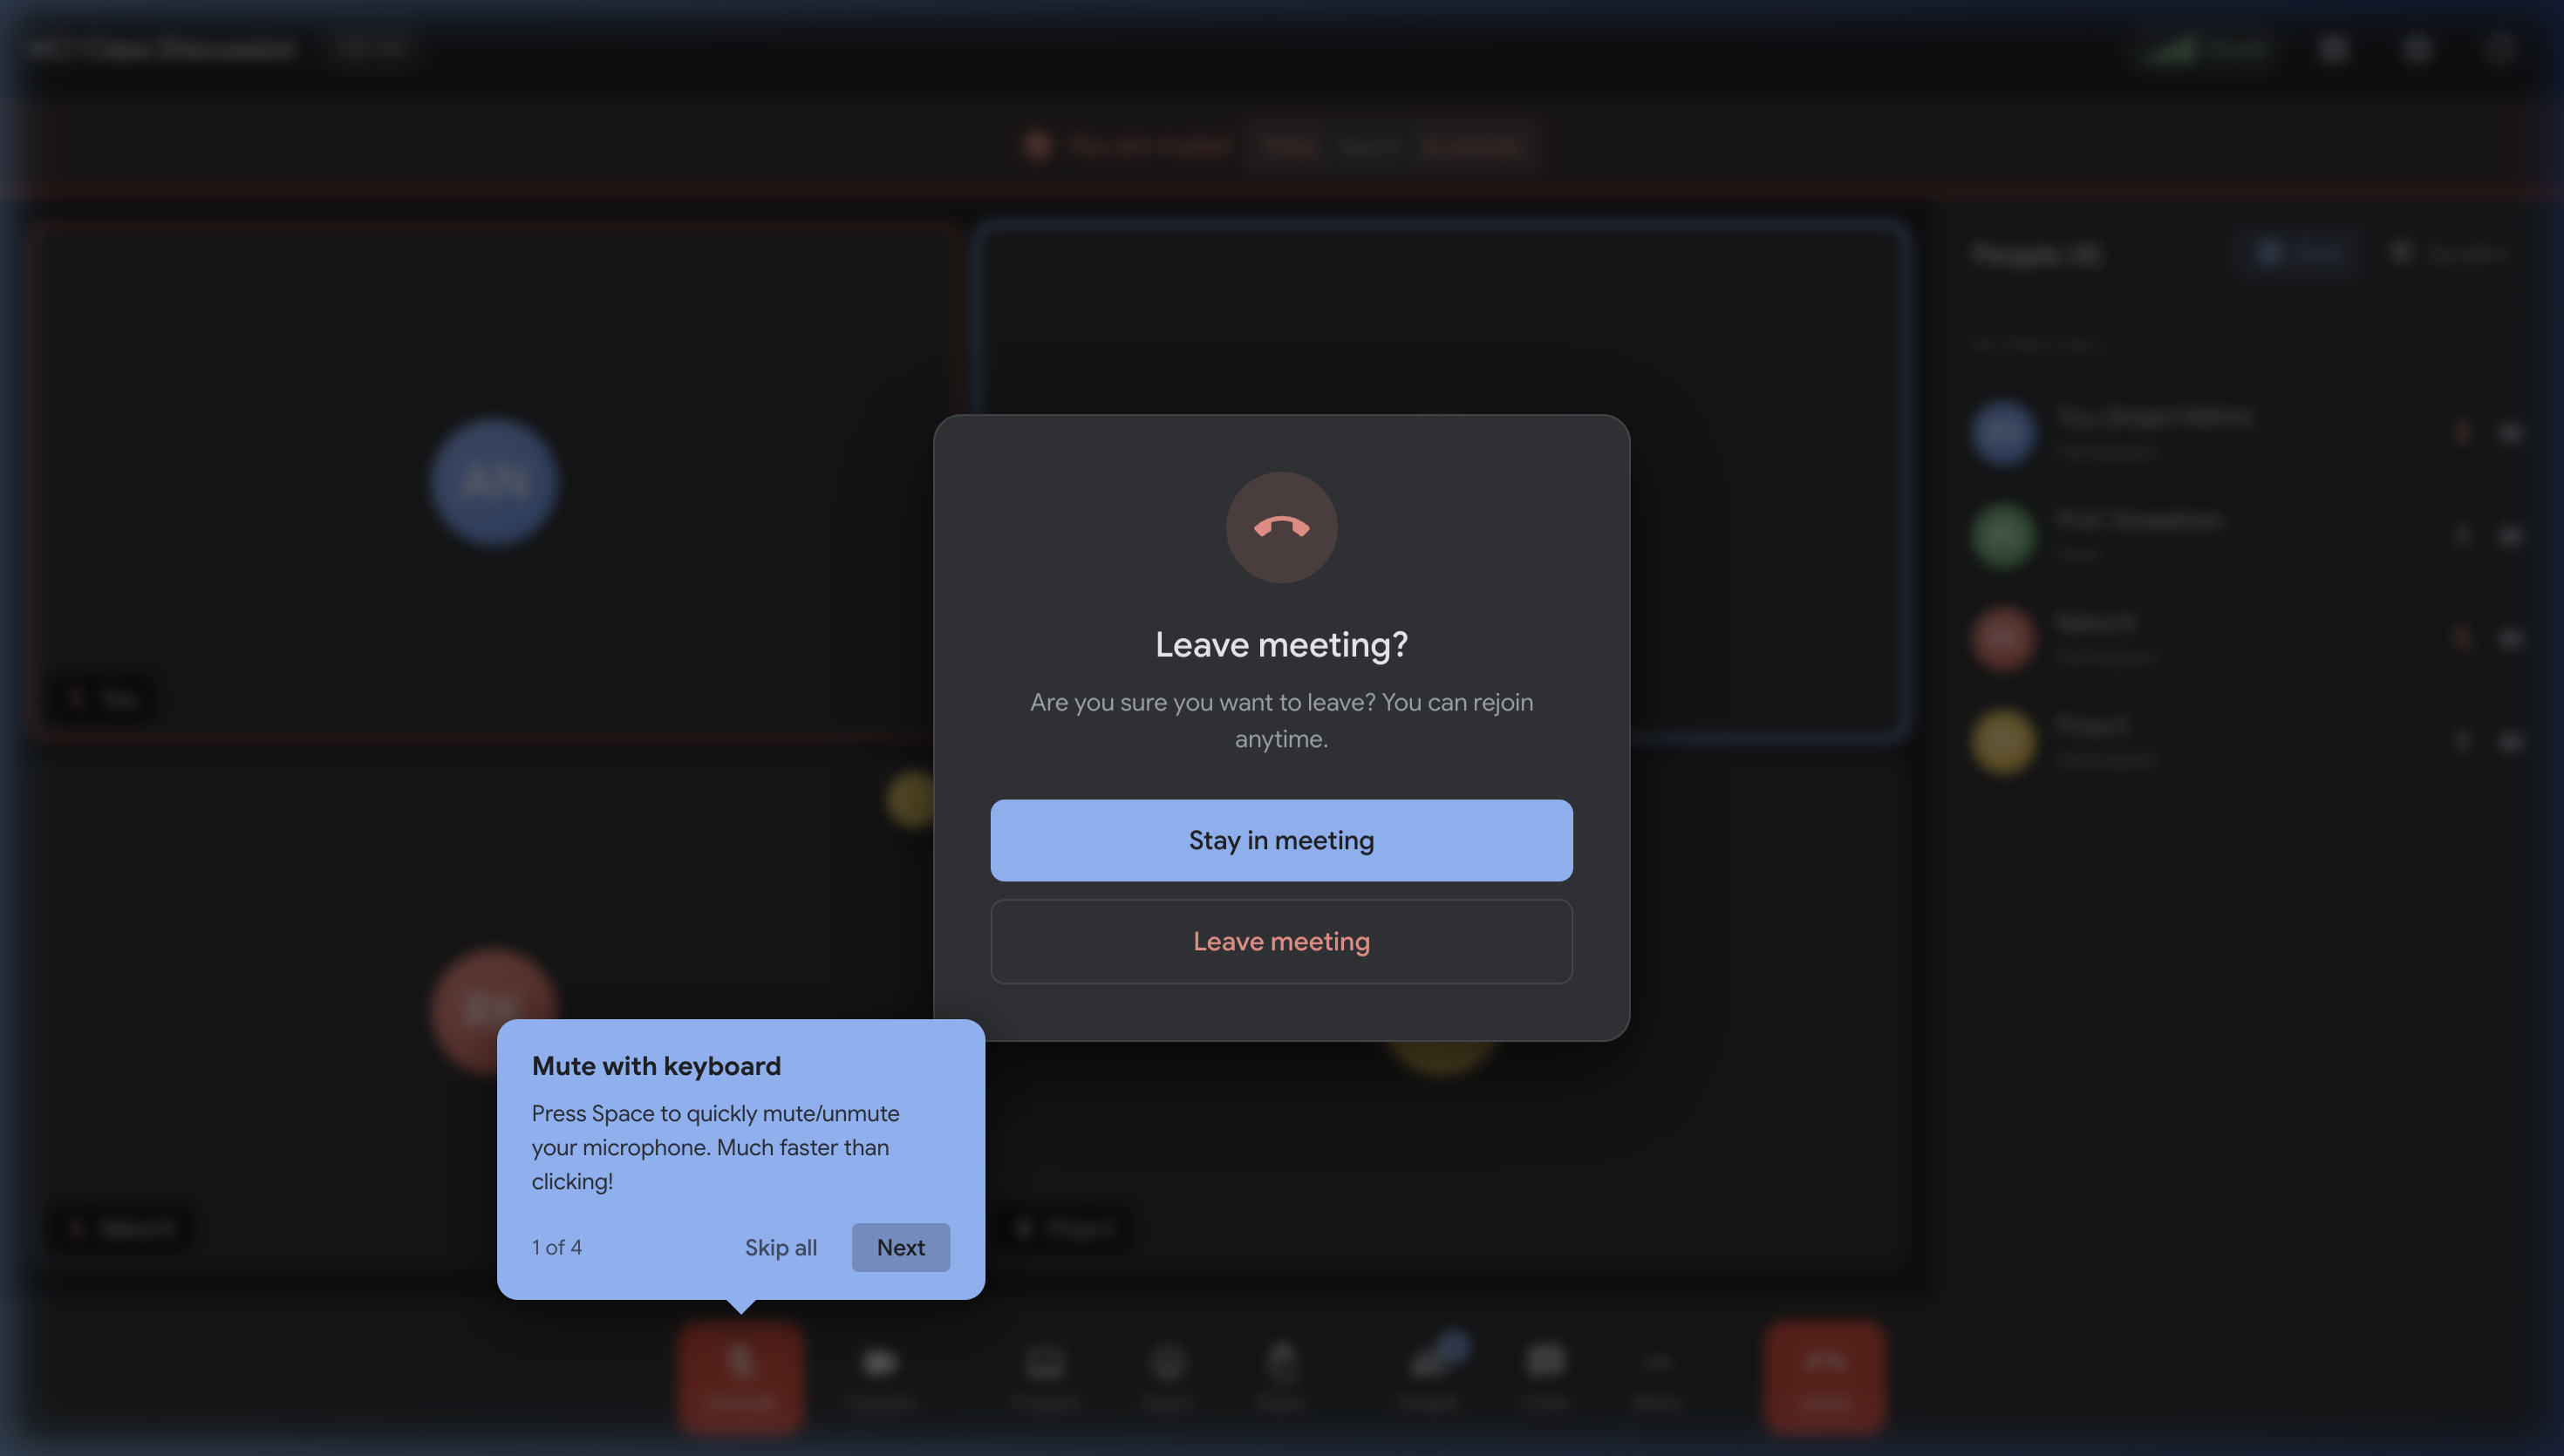
\includegraphics[width=0.8\textwidth]{images/leave_confirm.png}
    \caption{Leave Meeting Confirmatory Modal preventing accidental disconnection.}
\end{figure}

\subsubsection{Pre-Meeting Network Connection Check}
Before connecting to the main routing grid, users must pass through the \textbf{System Check Dashboard}. This visually verifies the Microphone, Camera, and Network Connection speed. This satisfies Nielsen \#1 (Visibility of System Status) and prevents the classic "Am I lagging?" error loop mid-meeting.

\begin{figure}[h]
    \centering
    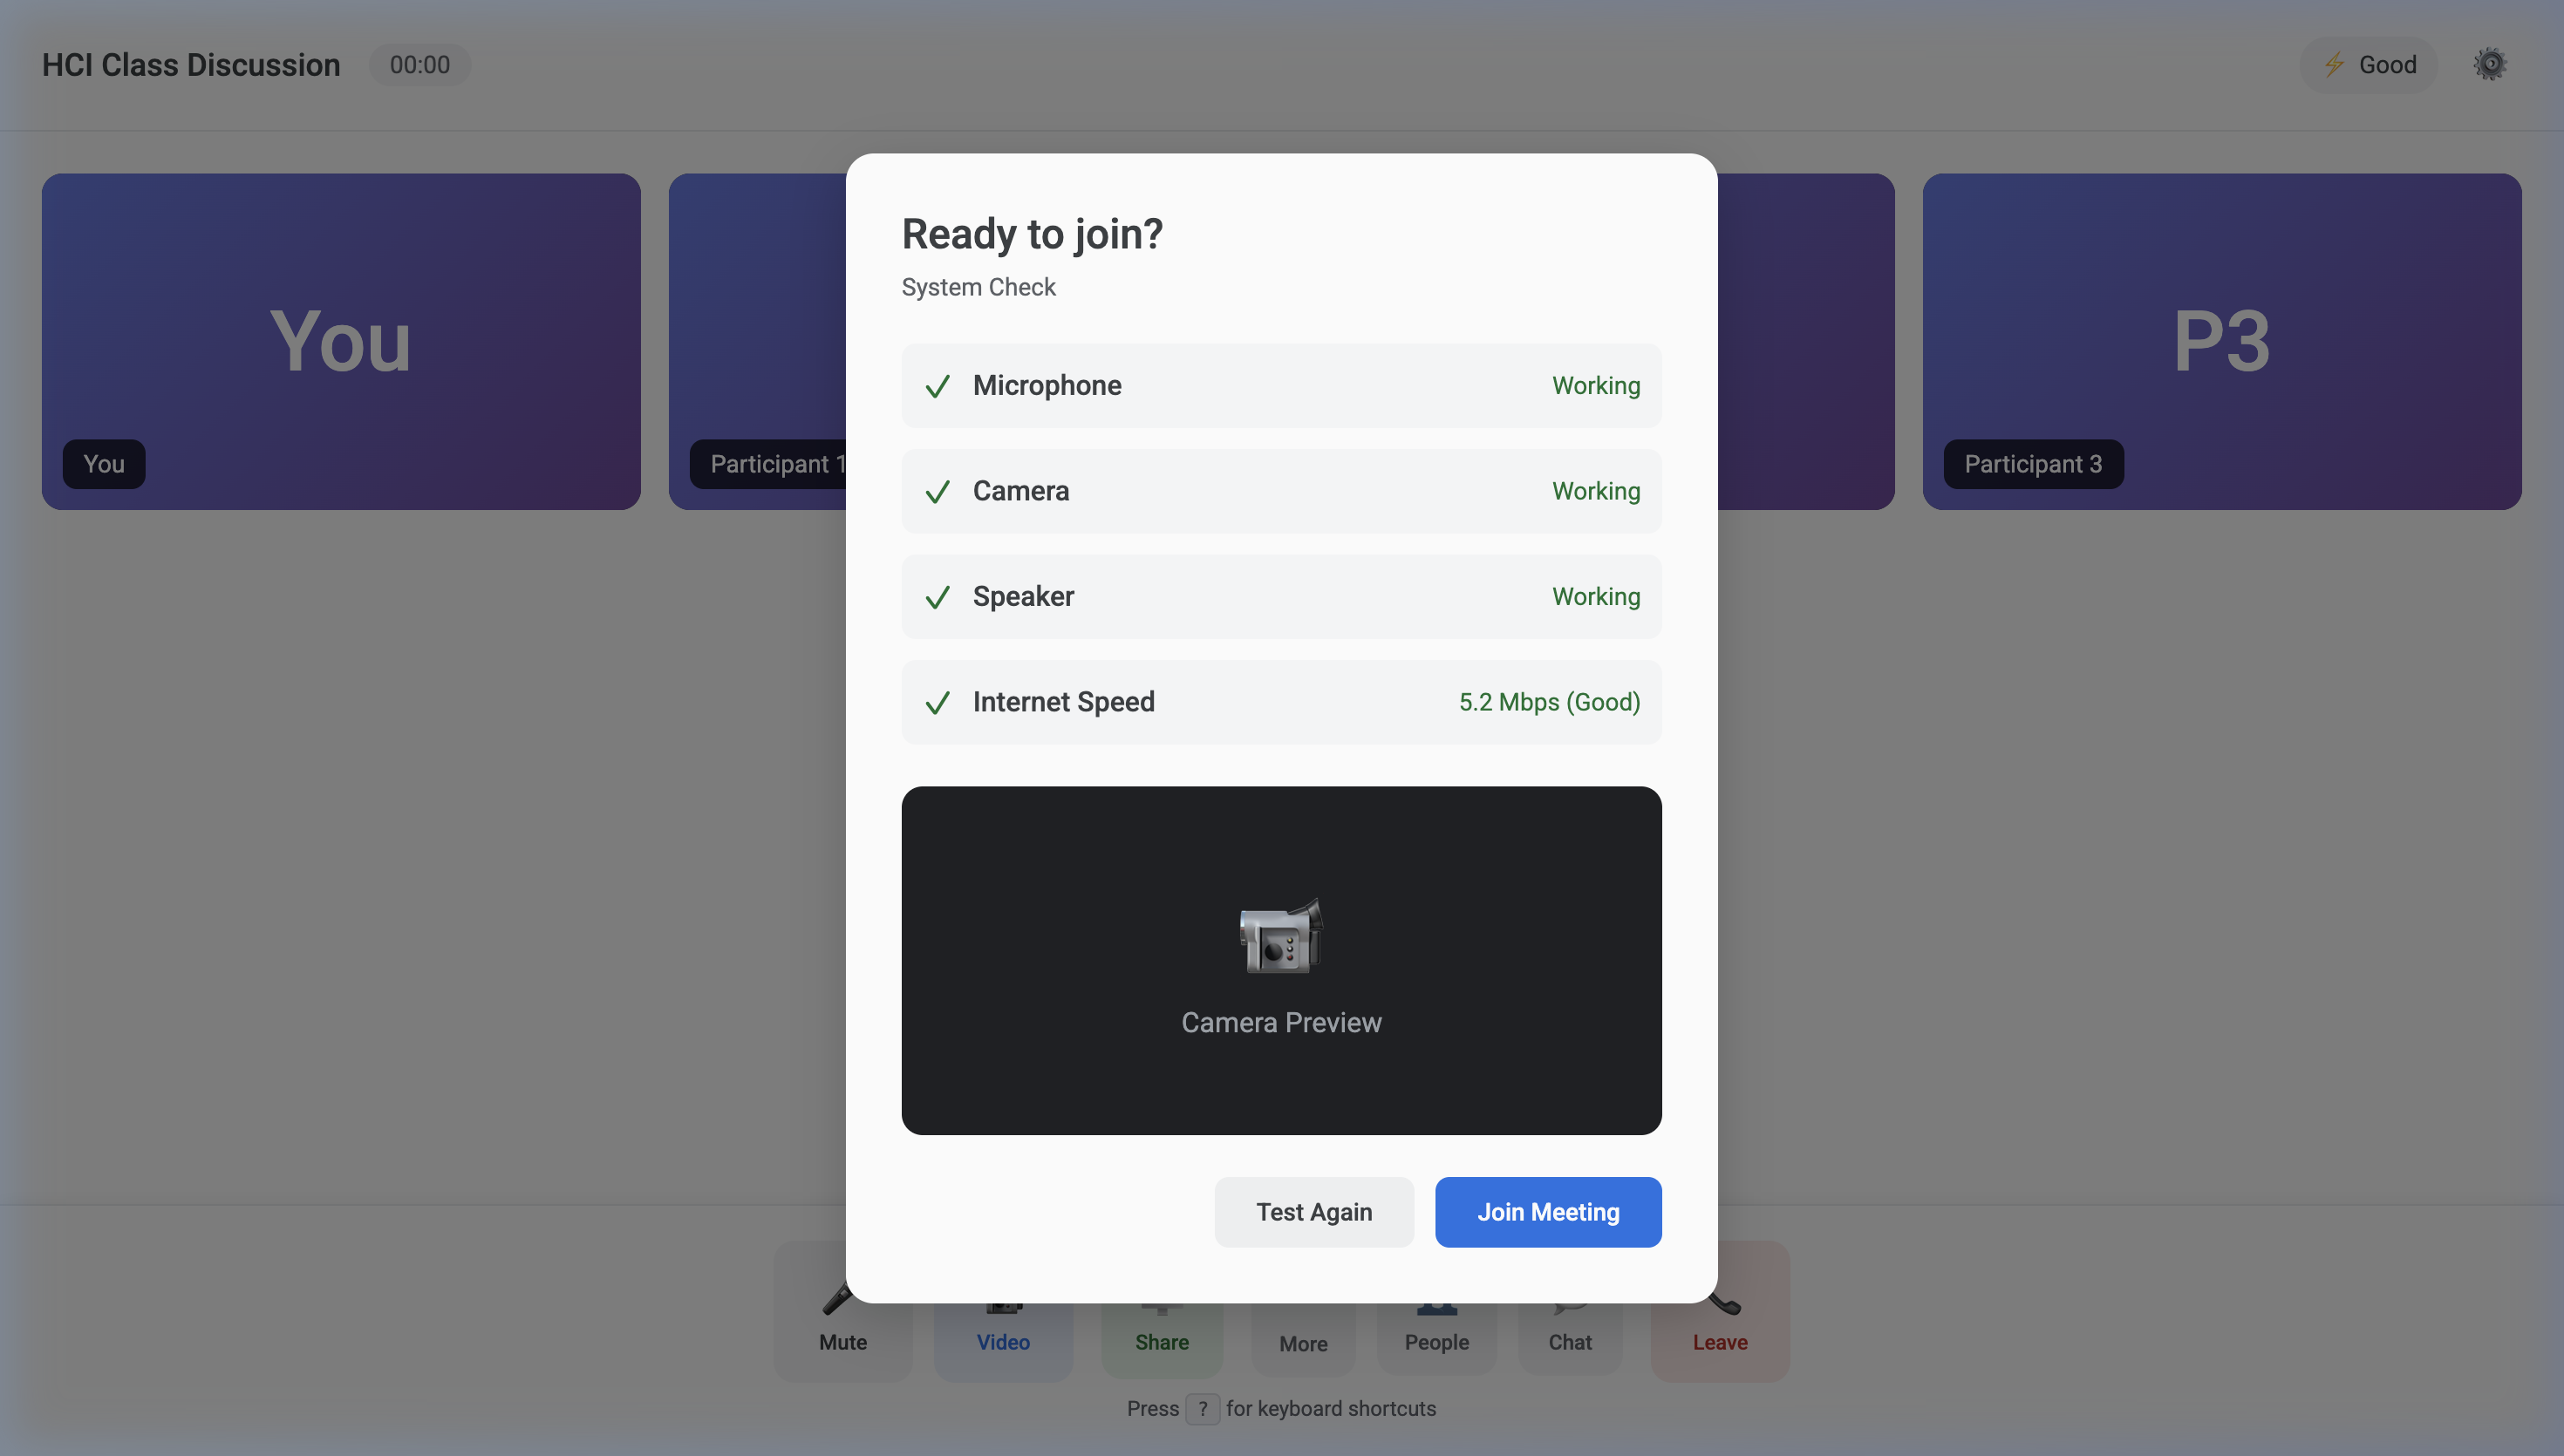
\includegraphics[width=0.8\textwidth]{images/pre_check.png}
    \caption{Pre-Meeting Dashboard checking Network and IO Devices.}
\end{figure}

\newpage
\subsection{Nielsen's Heuristic \#1: Visibility of System Status}

\subsubsection{Screen Share Feedback}
A major issue in modern WebRTC applications is the "Mirror Void" where users share their screen but cannot confirm the audience sees it. We built an overt \textbf{Screen Share Feedback Banner} that docks to the top of the grid and changes the user's local tile border to persistent Green, guaranteeing system status visibility.

\subsubsection{Multi-Modal Mute Feedback}
User's constantly forget their microphone state. We utilize Multi-Modal feedback to combat this. When muted, the system triggers three changes: a red "Muted" banner, a red border on the video tile, and the corresponding icon shift.

\begin{figure}[h]
    \centering
    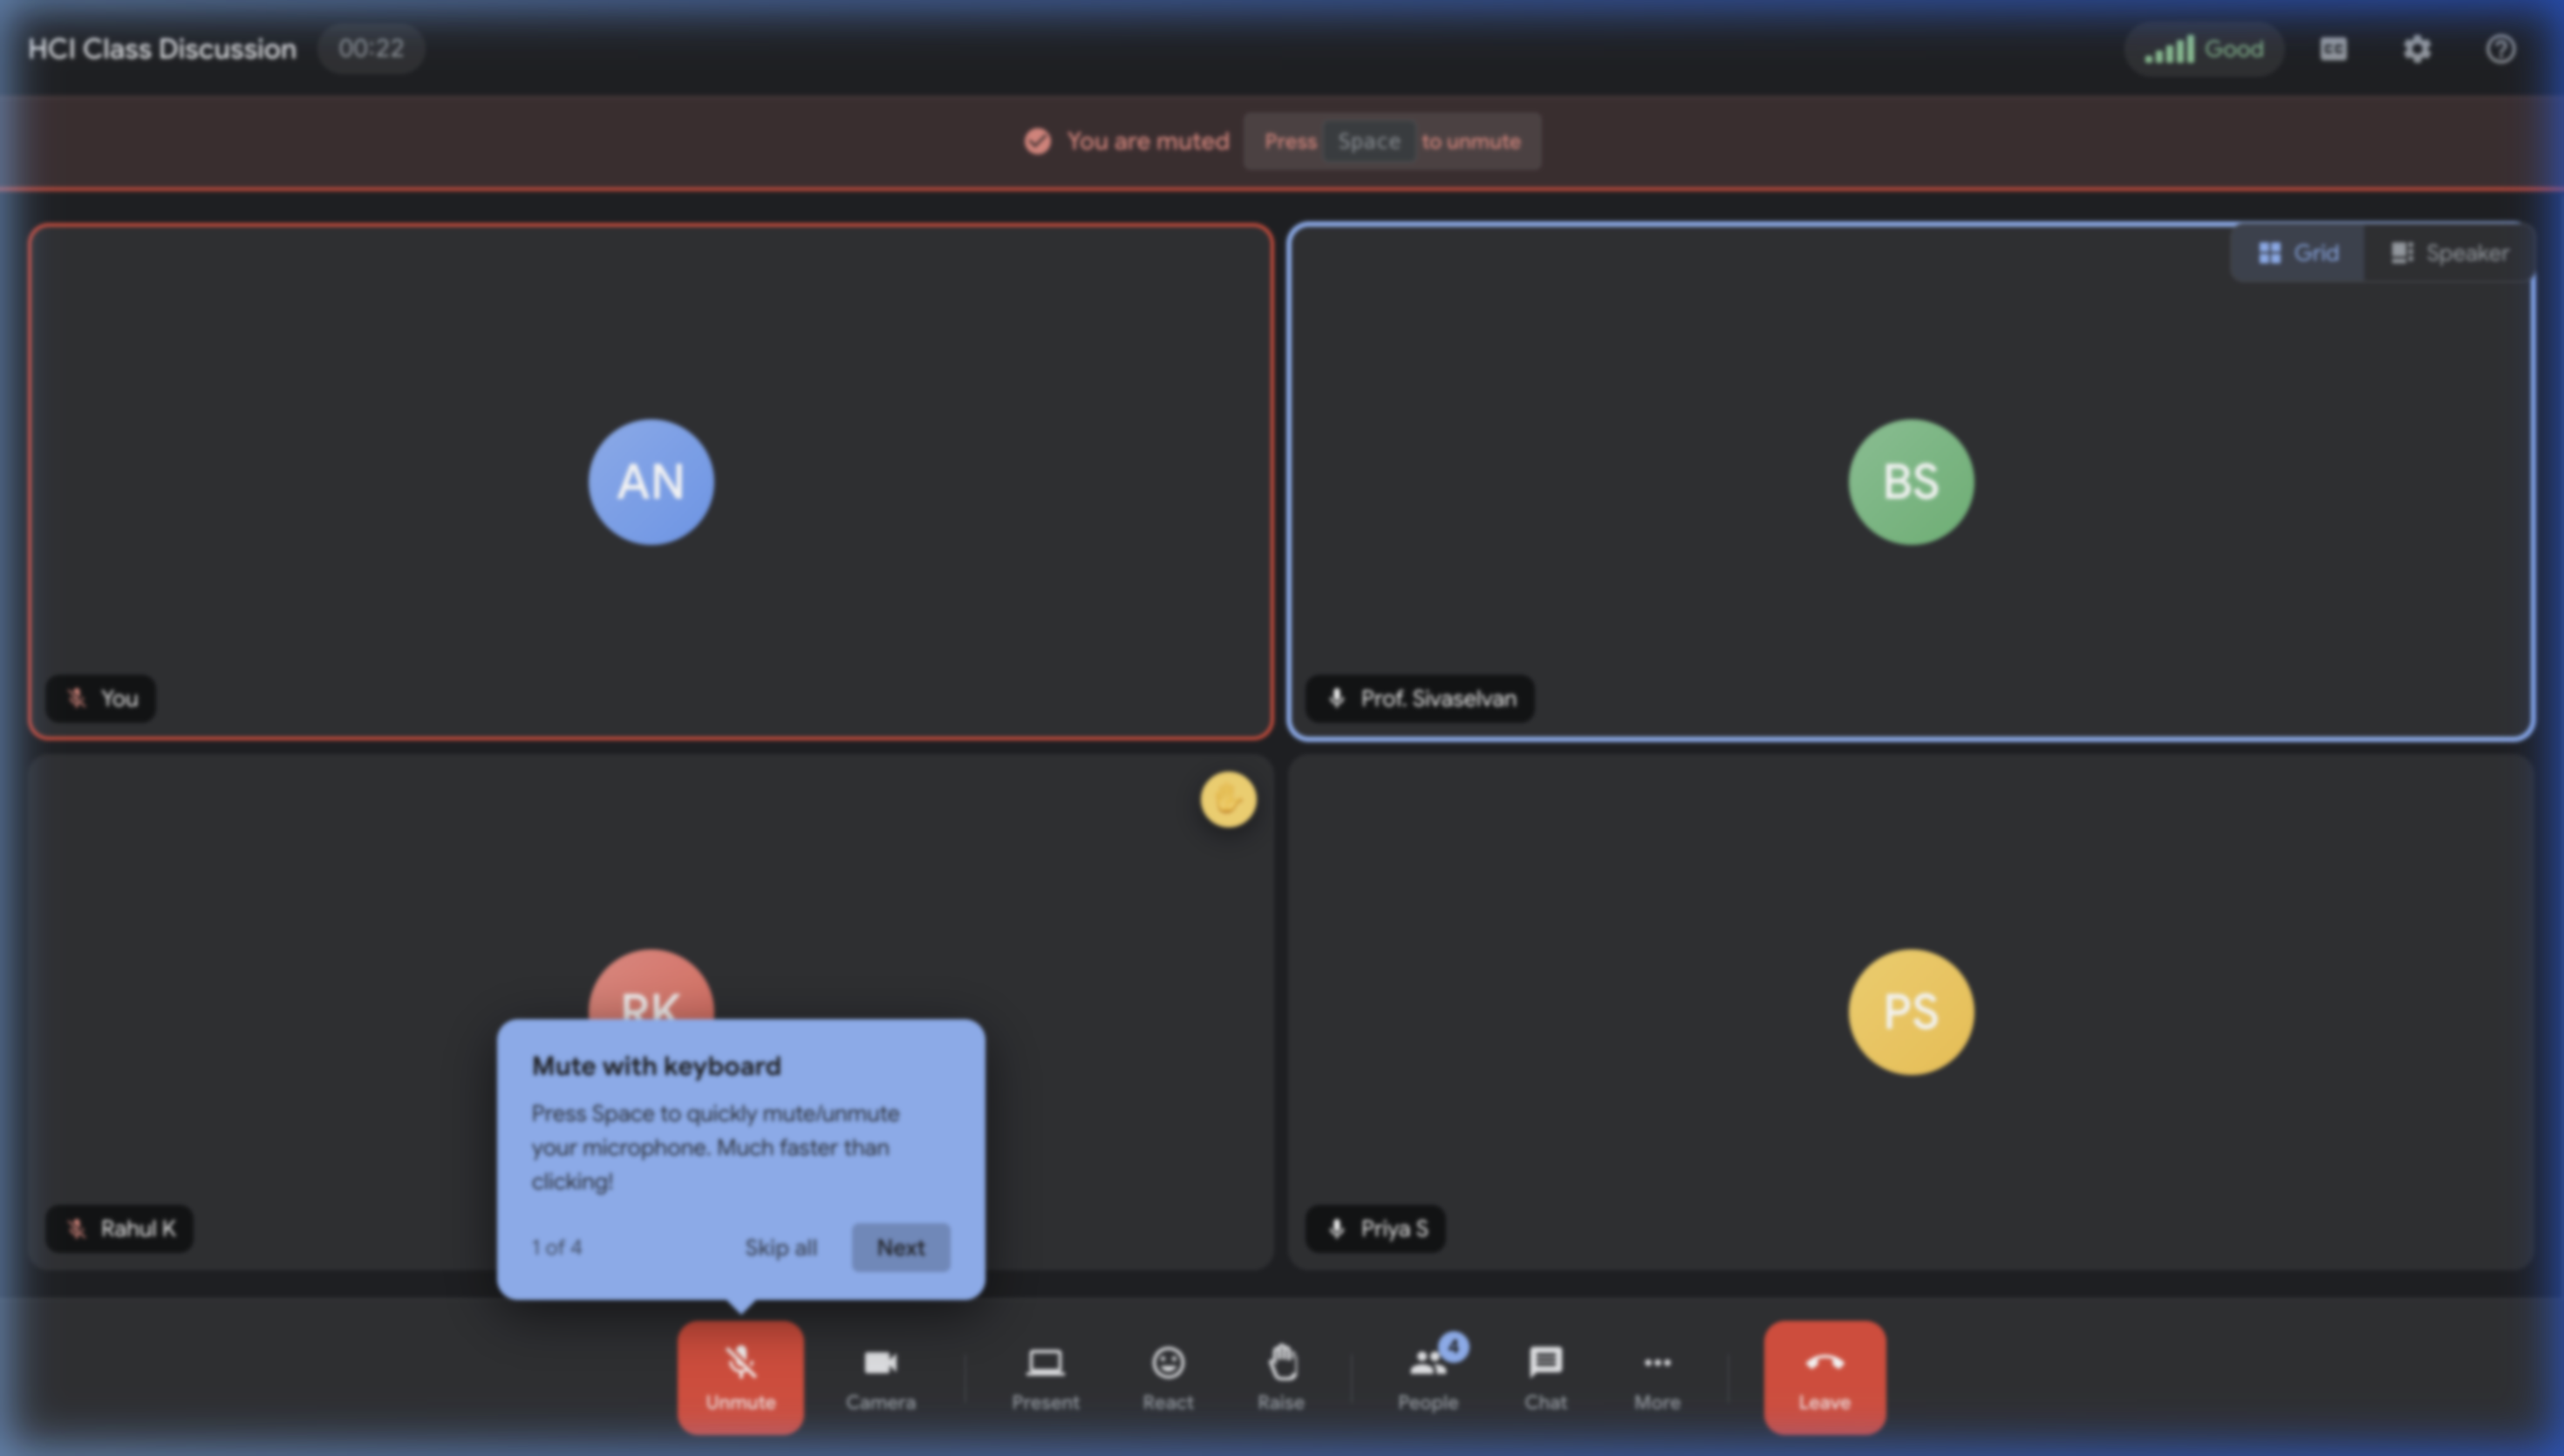
\includegraphics[width=0.8\textwidth]{images/mute_feedback.png}
    \caption{Tri-layered multi-modal feedback representing mute status securely.}
\end{figure}

\subsection{Nielsen's Heuristic \#3: User Control \& Freedom (Undo System)}
To provide a safety net, we implemented an \textbf{Undo Toast Notification}. If an action is accidentally fired (like dropping a screen share), the system offers a 4-second localized window to reverse the state action.

\begin{figure}[h]
    \centering
    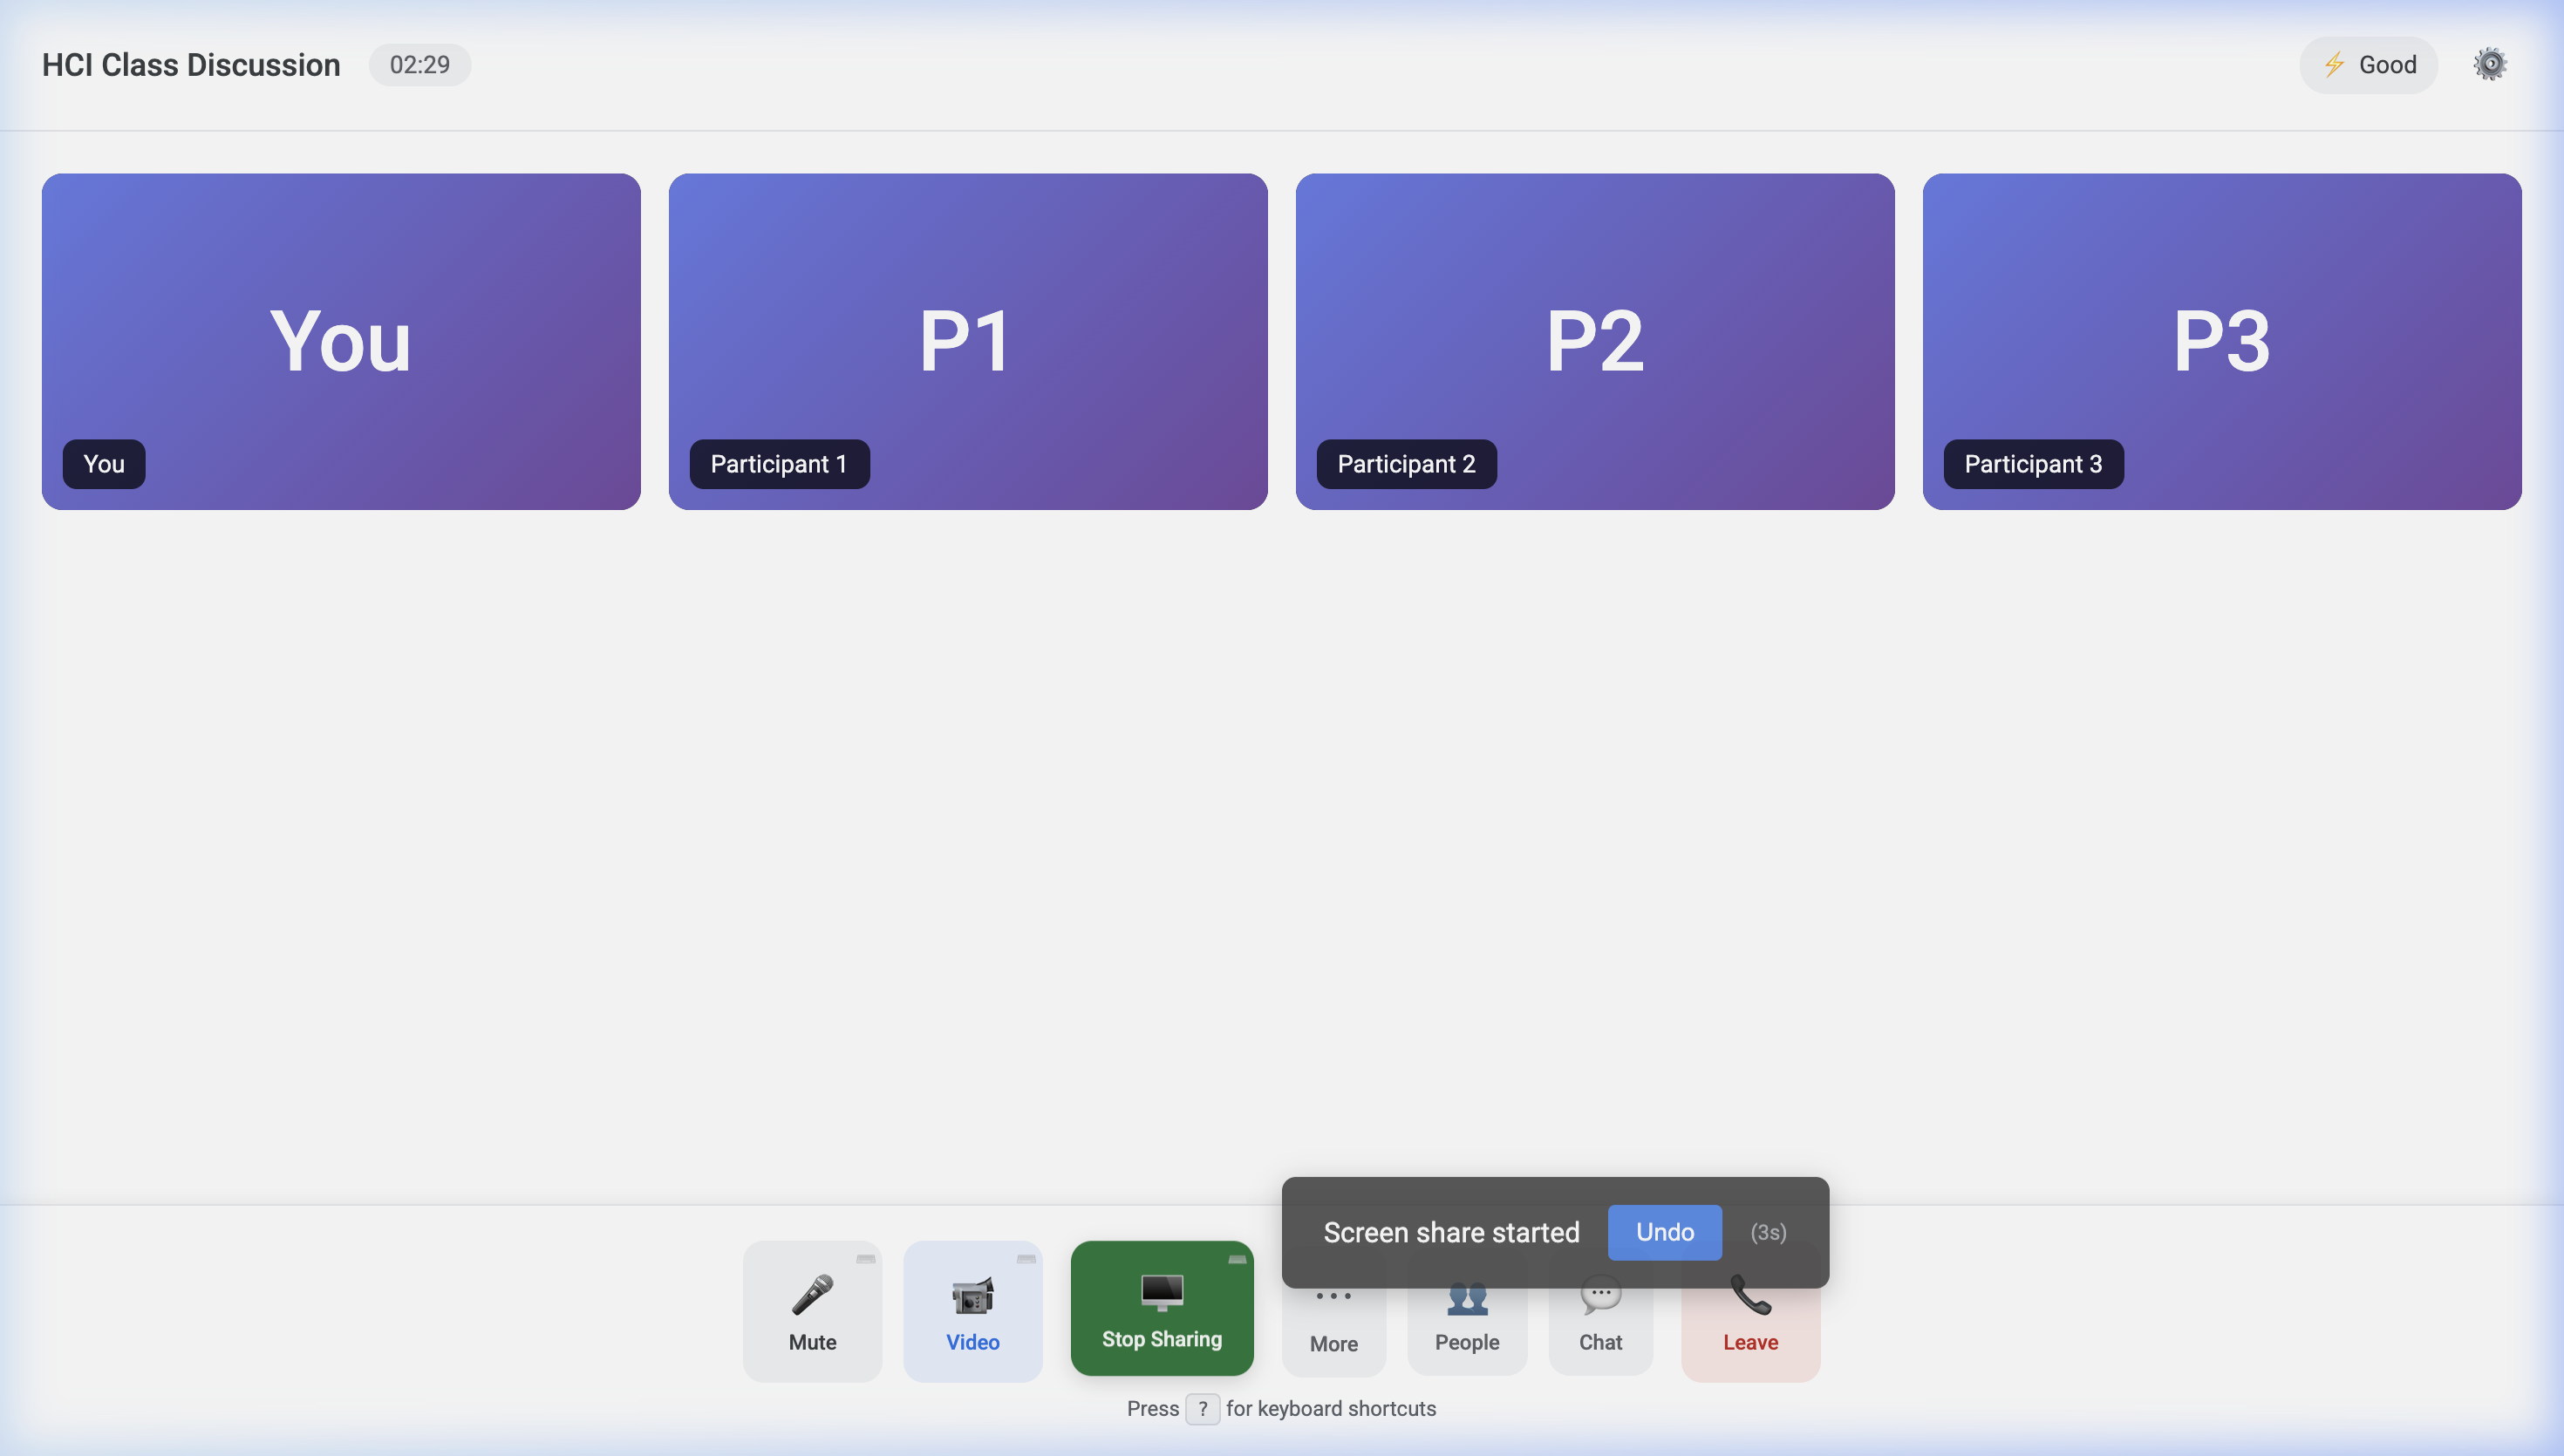
\includegraphics[width=0.8\textwidth]{images/undo_toast.png}
    \caption{The Undo System ensuring swift error recovery.}
\end{figure}

\newpage
\section{Learnability \& Flexibility Analysis}

\subsection{Learnability \& Predictability}
Learnability is defined by how easily a new user can achieve their goals on first interaction. We established learnability through strict visual mapping. 

\textbf{Color Coded Emphasis on Control Buttons:} Instead of monotone gray UI states, controls inherently define their function through color psychology:
\begin{itemize}
    \item \textbf{Red (Alert/Destructive):} Leave Meeting, Mute toggle active.
    \item \textbf{Green (Collaborative):} Screen share active.
    \item \textbf{Blue (Neutral/Focus):} General toggles, active speaker identification.
\end{itemize}

\begin{figure}[h]
    \centering
    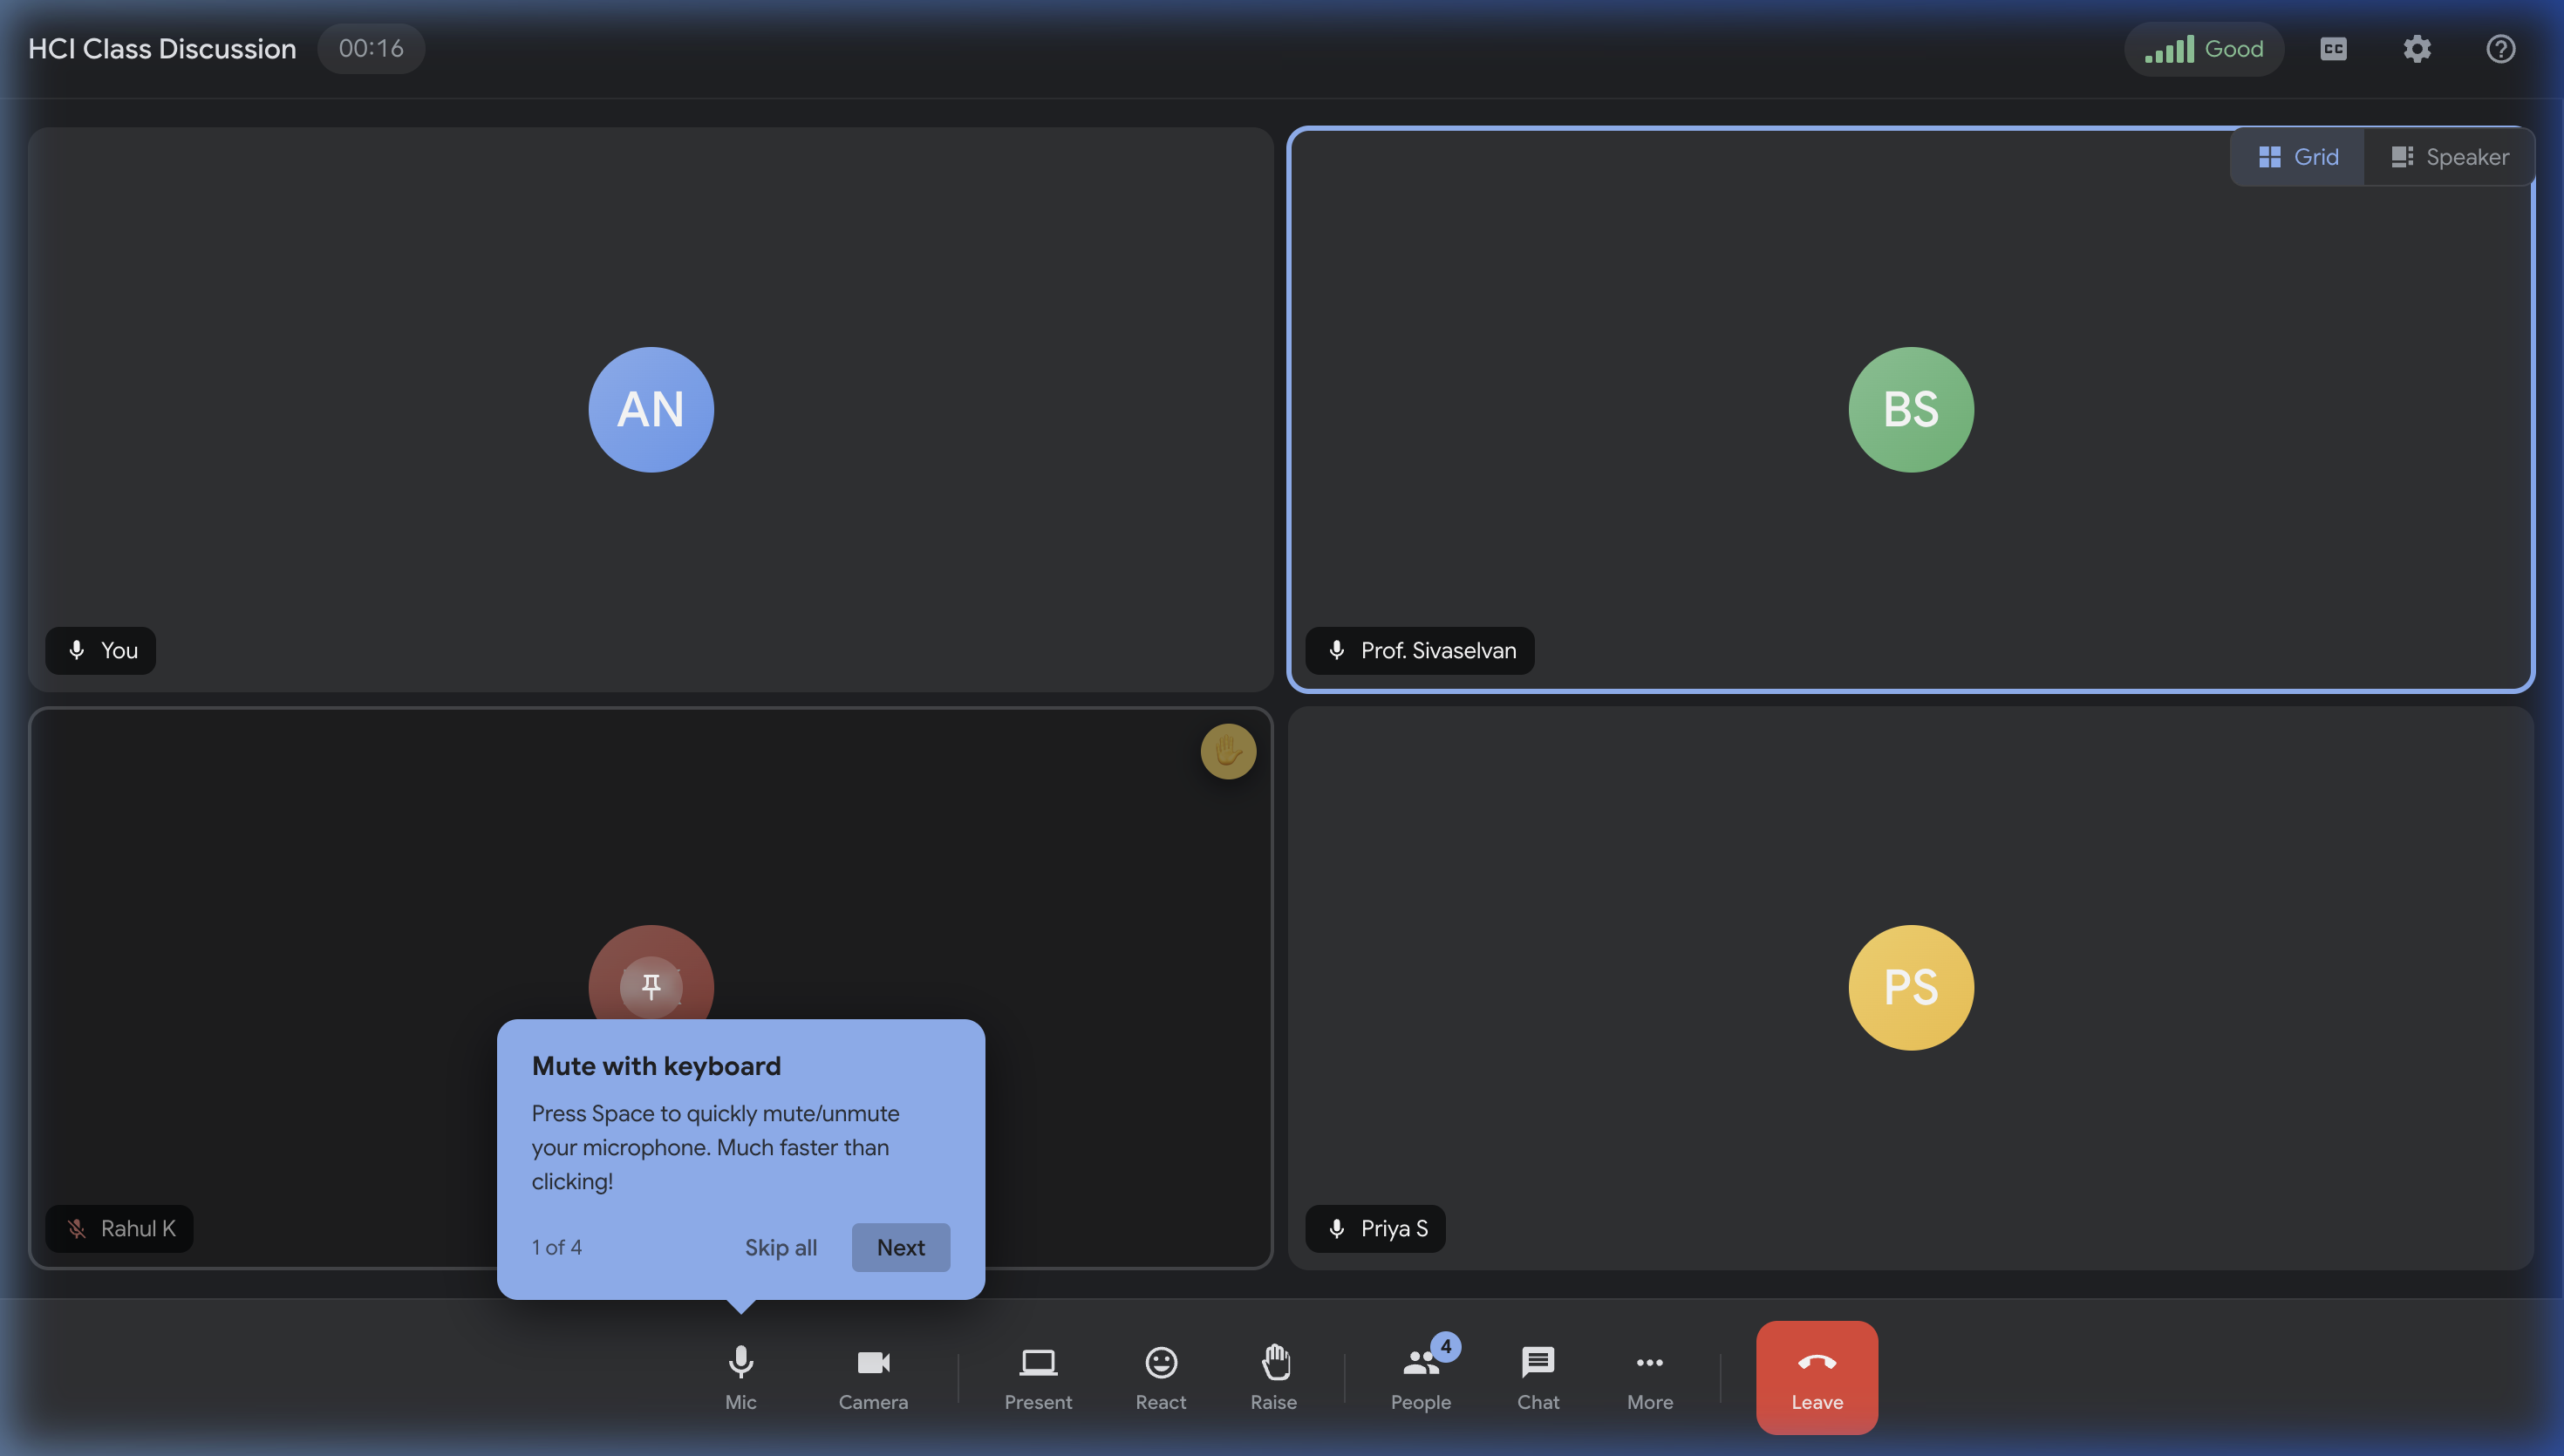
\includegraphics[width=0.8\textwidth]{images/main_ui.png}
    \caption{Color Coded Emphasis driving rapid learnability.}
\end{figure}

\subsection{Flexibility for Power Users}
Flexibility allows expert users to bypass tedious UI loops (Nielsen \#7). We achieved this by weaving \textbf{Keyboard Accelerators} into the core DOM context. Users can hit `Shift+?` to open a command palette, mapping global hotkeys like `Spacebar` for Quick-Mute effortlessly.

\section{Persuasive Psychology \& Nudge Theory}
Applying Robert Cialdini's principles, the dashboard onboarding now deeply employs:
\begin{itemize}
    \item \textbf{Social Proof:} Counters like ``14 students waiting'' prompt faster authentication action.
    \item \textbf{Reciprocity:} Our "Friendly Meeting Assistant" avatar preemptively suggests helpful actions (like lowering volume) before the user even asks.
    \item \textbf{Gamification/Consistency:} A post-meeting streak system uses commitment triggers to build positive habits over recurring sessions.
\end{itemize}

\section{Conclusion}
This redesign intentionally pivots away from theoretical block diagrams and textual descriptions into actively implemented, high-fidelity UI solutions. By strictly coupling actual interface elements with Fitts's Law, error prevention schemas, and flexible control systems, this platform synthesizes the core psychological comfort necessary for an optimal conferencing environment.

\end{document}
